%  This document is generated by `src/word-embeddings-figure.py`
%  Please do not edit it directly as it will be likely overwritten
%  The figure represents a Hasse diagram of a relation between words
%  The words are represented as nodes and the relation as edges
%  The figure is generated using TikZ and can be included in a LaTeX document
%  using the `standalone` class/package.
\documentclass[tikz]{standalone}
\usepackage{tikz}
\usepackage{ensps-colorscheme}
\begin{document}
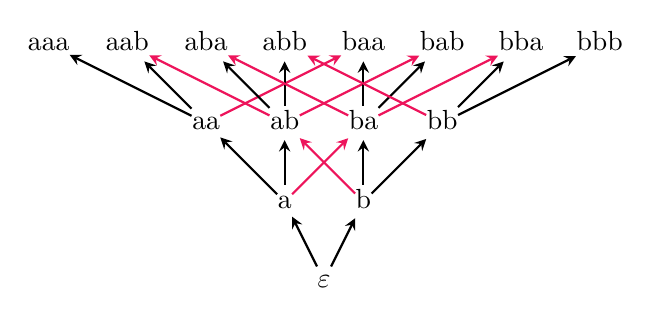
\begin{tikzpicture}[
        isWord/.style={rectangle,inner sep=0mm},
        isEmbedding/.style={->, >=stealth, thick},
        branch/.style={A5},
        antichain/.style={A2},
        branchEdge/.style={A5,dashed},
        outEdge/.style={dotted,B2},
        isInfixEnc/.style={},
        isRealWord/.style={A4,opacity=0.2},
        isRealEmbedding/.style={A4,opacity=0.2},
        isNewEdge/.style={B2},
        ]

        
\node[isWord] (epsilon) at (-0.5, 0) {\strut $\varepsilon$};
\node[isWord] (a) at (-1.0, 1) {\strut a};
\node[isWord] (b) at (0.0, 1) {\strut b};
\node[isWord] (aa) at (-2.0, 2) {\strut aa};
\node[isWord] (ab) at (-1.0, 2) {\strut ab};
\node[isWord] (ba) at (0.0, 2) {\strut ba};
\node[isWord] (bb) at (1.0, 2) {\strut bb};
\node[isWord] (aaa) at (-4.0, 3) {\strut aaa};
\node[isWord] (aab) at (-3.0, 3) {\strut aab};
\node[isWord] (aba) at (-2.0, 3) {\strut aba};
\node[isWord] (abb) at (-1.0, 3) {\strut abb};
\node[isWord] (baa) at (0.0, 3) {\strut baa};
\node[isWord] (bab) at (1.0, 3) {\strut bab};
\node[isWord] (bba) at (2.0, 3) {\strut bba};
\node[isWord] (bbb) at (3.0, 3) {\strut bbb};
\draw[isEmbedding] (epsilon) -- (a);
\draw[isEmbedding] (epsilon) -- (b);
\draw[isEmbedding] (a) -- (aa);
\draw[isEmbedding] (a) -- (ab);
\draw[isEmbedding,isNewEdge] (a) -- (ba);
\draw[isEmbedding,isNewEdge] (b) -- (ab);
\draw[isEmbedding] (b) -- (ba);
\draw[isEmbedding] (b) -- (bb);
\draw[isEmbedding] (aa) -- (aaa);
\draw[isEmbedding] (aa) -- (aab);
\draw[isEmbedding,isNewEdge] (aa) -- (baa);
\draw[isEmbedding,isNewEdge] (ab) -- (aab);
\draw[isEmbedding] (ab) -- (aba);
\draw[isEmbedding] (ab) -- (abb);
\draw[isEmbedding,isNewEdge] (ab) -- (bab);
\draw[isEmbedding,isNewEdge] (ba) -- (aba);
\draw[isEmbedding] (ba) -- (baa);
\draw[isEmbedding] (ba) -- (bab);
\draw[isEmbedding,isNewEdge] (ba) -- (bba);
\draw[isEmbedding,isNewEdge] (bb) -- (abb);
\draw[isEmbedding] (bb) -- (bba);
\draw[isEmbedding] (bb) -- (bbb);

\end{tikzpicture}
\end{document}
        
